\documentclass[12pt,a4paper,twoside,final]{book} %% PRO OBOUSTRANNY TISK -> twoside

\usepackage{mypackage} % moje definice a styly

\usepackage{cool}
\Style{DSymb={\mathrm d},DShorten=true,IntegrateDifferentialDSymb=\mathrm{d}}

\faculty{Faculty of science}
\department{Department of theoretical physics and astrophysics}
\university{Masaryk University}
\thesisType{Ph.D. Dissertation}
\city{Brno}
\academicYear{2021/2022}
\yearOfMaking{2022}

% vícejazyčný název práce
\thesisTitle{Analysis and Modeling of Nonlinear \newline Dynamical Systems in Astrophysics}
\thesisTitleEN{Analysis and Modeling of Nonlinear \newline Dynamical Systems in Astrophysics}
\thesisTitleCZ{Analýza a modelování nelineárních dynamických systémů v astrofyzice}

\author{Mgr. Jiří Květoň}
\supervisor{Mgr. Filip Hroch Ph.D.}
\consultant{Mgr. Viktor Votruba Ph.D.}

\coverImage{img/cover.png}

% References package defs
\usepackage[
    backend=biber,
    style=authoryear,
    citestyle=authoryear,
    sorting=ynt
]{biblatex}

% References file
% pozn. https://tex.stackexchange.com/questions/305381/biblatex-empty-bibliography ... kvuli chybe nedefinovanych bib
\addbibresource{./references.bib}

\usepackage{hyperref}
\hypersetup{colorlinks=true,allcolors=black}
\usepackage{hypcap}

\begin{document}
    % Pro uvodni strany se vypne cislovani
    \pagenumbering{gobble}

    % --
    % Titulní strana prace
    % --
    \maketitle

    % --
    % Originální zadání
    % --
    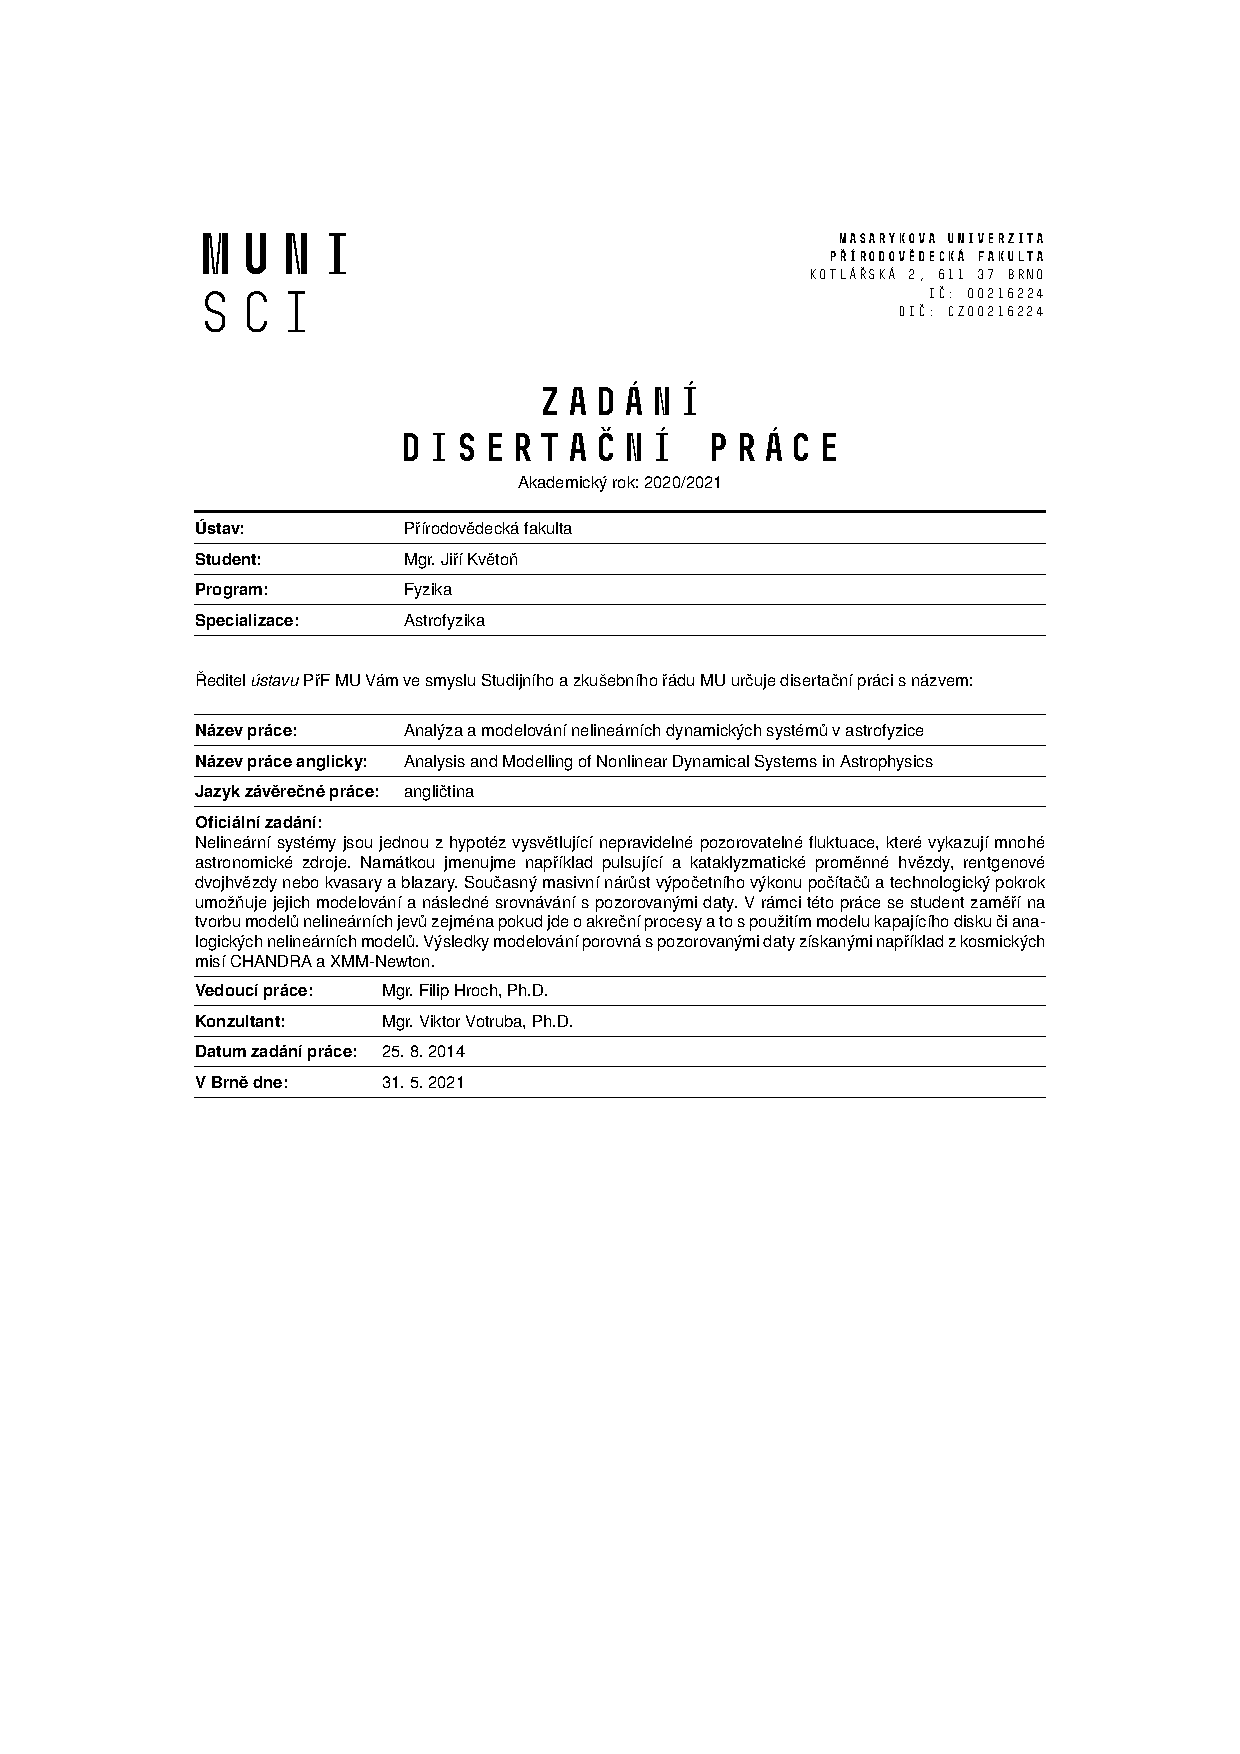
\includepdf{./zadani.pdf}

    \pagestyle{plain}

    % --
    % Obsah
    % --
    \frontmatter
    \pagenumbering{gobble}
    \tableofcontents
    \mainmatter

    \pagenumbering{roman}
    \setcounter{page}{1}

    % --
    % Bibliografický záznam
    % --
    \phantomsection
    \bibinfoen

    \phantomsection
    \bibinfocz

    % --
    % Abstrakt (CZ+EN)
    % --
    \phantomsection
    \shortchapter{abstract}{abstract-en.tex}

    \phantomsection
    \shortchapter{abstrakt}{abstract-cz.tex}

    % --
    % Poděkování
    % --
    \phantomsection
    \shortchapter{acknowledgments}{acknowledgments.tex}

    % --
    % Prohlášení
    % --
    \phantomsection
    \declaration{declaration.tex}

    % Zapnout cislovani a vlastni styl hlavniho obsahu
    \pagenumbering{arabic}
    \setcounter{page}{1}
    \pagestyle{mystyle}

    % --
    % Kapitoly
    % --

    % 1. INTRODUCTION
    % ...
    \chapter{INTRODUCTION}
\thispagestyle{empty}


    %%%%%%%%%%%%%%%%%%%
    % TEORETICKÁ ČÁST %
    %%%%%%%%%%%%%%%%%%%

    % 2. ACCRETION DISCS
    \chapter{ACCRETION DISCS}
\thispagestyle{empty}


    % 3. FLICKERING PHENOMENON
    \chapter{\color{red}FLICKERING PHENOMENON}
\thispagestyle{empty}


    % 4. CATACLYSMIC VARIABLES
    \chapter{CATACLYSMIC VARIABLES}
\thispagestyle{empty}


    % 5. SIMILARITY OF NON-LINEAR SYSTEMS
    \chapter{\color{red}SIMILARITY OF NON-LINEAR SYSTEMS}
\thispagestyle{empty}



    % 6. DRIPPING FAUCET
    \chapter{DRIPPING FAUCET}

\section{Basics}
\section{Fluid dynamical model (FDM)}
\section{Mass-spring model (MSM)}

\thispagestyle{empty}


    % 7. DRIPPING HANDRAIL MODELS
    \chapter{DRIPPING HANDRAIL MODELS}
\thispagestyle{empty}


    % 8. MODELING TECHNIQUES
    \chapter{\color{red}MODELING TECHNIQUES}
\thispagestyle{empty}


    %%%%%%%%%%%%%%%%%%
    % PRAKTICKÁ ČÁST %
    %%%%%%%%%%%%%%%%%%

    % 9. MDH - MODEL PROPOSAL 
    \chapter{MDH -- MODEL PROPOSAL}
\thispagestyle{empty}

I propose a model constructed of \emph{n} times \emph{m} individual cells arranged in multi-layer ringlike structure. Each layer (i.e. ring) is denoted by $i \in [0; n-1]$, with the outermost layer having $i = 0$ and cells in each layer are denoted by $j \in [0; m-1]$ \footnote{Direction of $j$ iteration is arbitrary and a matter of perspective (i.e top vs. bottom view).}. Each cell holds a set of parameters and its behavior is governed by set of oridinary differential equations derived from Mass-Spring model so fundamentally every cell is its own \emph{dripping faucet} system so lets start by defining individual cell.  

\section{Cell definition}
The imagined cell holds following set of parameters:

\begin{center}
\begin{tabular}{r|l}
$i$			& Layer index \\
$j$			& Cell index \\
$r$			& Orbital radius \\
$\theta$	& Orbital azimuth \\ 
$z$			& Mass spring model \emph{spring elongation}  \\
$v$			& Mass-Spring model \emph{velocity} \\
$m$			& Mass contained by cell \\
$\Delta m$ 	& Mass change since previous step \\
$g$			& Gravitational acceleration relative to outermost layer \\
$\gamma$	& Constant Mass-Spring model dumpening parameter \\
$k$			& Mass-Spring model \emph{spring stiffness} \\
$T$			& Cell temperature \\ 
\end{tabular}
\end{center}

\subsection{Coordinate system and indexing}

\subsection{Orbital radius and azimuth}

\subsection{Temperature}



\section{}


    % 10. MULTILAYER DRIPPING HANDRAIL - MODEL IMPLEMENTATION 
    \chapter{MDH -- MODEL IMPLEMENTATION}
\thispagestyle{empty}


    % 11. MULTILAYER DRIPPING HANDRAIL - DATA ANALYSIS
    \chapter{\color{red}MDH -- DATA ANALYSIS}
\thispagestyle{empty}


    % 12. MULTILAYER DRIPPING HANDRAIL - OBSERVATIONAL DATA CONFRONTATION  
    \chapter{MDH -- OBSERVATIONAL DATA CONFRONTATION}
\thispagestyle{empty}



    % 13. DISCUSSION
    \chapter{\color{red}DISCUSSION}


    \pagestyle{plain}

    % Seznam použitých zkratek
    \newpage
    \phantomsection
    \addcontentsline{toc}{chapter}{LIST OF ABBREVIATIONS}
    \noindent \Large \textbf{LIST OF ABBREVIATIONS}
    \normalsize
    \vspace{1cm}

\begin{center}
\def\arraystretch{1.5}%
\setlength\tabcolsep{1cm}
\begin{tabular}{ll}

CV			& Cataclysmic Variable star \\
WD			& White Dwarf star \\
FDM			& Fluid Dynamical Model \\
MSM			& Mass-Spring Model \\
MSMM			& Mass-Spring Model Modified \\
CA			& Cellular automaton \\
ODE			& Drdinary Differential Equation

\end{tabular}
\end{center}

    % Seznam použitých konstant
    \newpage
    \phantomsection
    \addcontentsline{toc}{chapter}{LIST OF CONSTANTS}
    \noindent \Large \textbf{LIST OF CONSTANTS}
    \normalsize
    \newpage

\phantomsection
\addcontentsline{toc}{chapter}{LIST OF CONSTANTS}
\noindent \Large \textbf{LIST OF CONSTANTS}
\normalsize

\vspace{10mm}
\begin{center}

\begingroup
\def\arraystretch{1.5}

\begin{tabularx}{\textwidth}{ccX}
\hline
\hline
\textbf{Symbol}	& \textbf{Value [units]} & \textbf{Meaning} \\
\hline
\hline
$G$	&
	\begin{tabular}{c}
		 $6.67430 \cdot 10^{-11}\ [N \cdot m^2 \cdot kg^{-2}]$ \\
		 $6.67430 \cdot 10^{-8}\ [dyne \cdot cm^2 \cdot g^{-1}]$
	\end{tabular} 
	& Gravitational const. \\

$h$ &
	\begin{tabular}{c}
		 $...$ \\
		 $6.6260755 \cdot 10^{-27}\ [cm^2 \cdot g \cdot s^{-1}]$
	\end{tabular} 
	& Planck's const. \\
	
$k$ &
	\begin{tabular}{c}
		 $...$ \\
		 $1.380658 \cdot 10^{-16}\ [erg \cdot K^{-1}]$
	\end{tabular} 
	& Boltzmann's const. \\
	
$\sigma$ &
	\begin{tabular}{c}
		 $...$ \\
		 $5.670374 \cdot 10^{-5}\ [erg \cdot cm^{-2} \cdot g^{-1} \cdot s^{-2}]$
	\end{tabular} 
	& Stefan-Boltzmann's const. \\

$c$ &
	\begin{tabular}{c}
		 $2.99792458 \cdot 10^{8}\ [m \cdot s^{-1}]$ \\
		 $2.99792458 \cdot 10^{10}\ [cm \cdot s^{-1}]$
	\end{tabular} 
	& Speed of light \\
	
	
$M_{\odot}$	&
	\begin{tabular}{c}
		 $1.98847\cdot 10^{30}\ [kg]$ \\
		 $1.98847\cdot 10^{33}\ [g]$
	\end{tabular} 
	& Solar mass \\
	
\hline

\end{tabularx}

\endgroup

\end{center}


    % --
    % Seznam literatury
    % -- 
    \newpage
    \phantomsection
    \addcontentsline{toc}{chapter}{REFERENCES}
    \noindent \Large \textbf{REFERENCES}
    \printbibliography[type=article,title={Articles},heading=subbibliography]
    \printbibliography[type=book,title={Books},heading=subbibliography]
    \printbibliography[type=misc,title={Miscellaneous},heading=subbibliography]
\end{document}
